\chapter{Arrays of Objects}

\section{Exercises}

\begin{exercise}
Consider this UML diagram for a \java{City} class in Figure~\ref{fig.cityuml}

\begin{figure}[!h]
\begin{center}
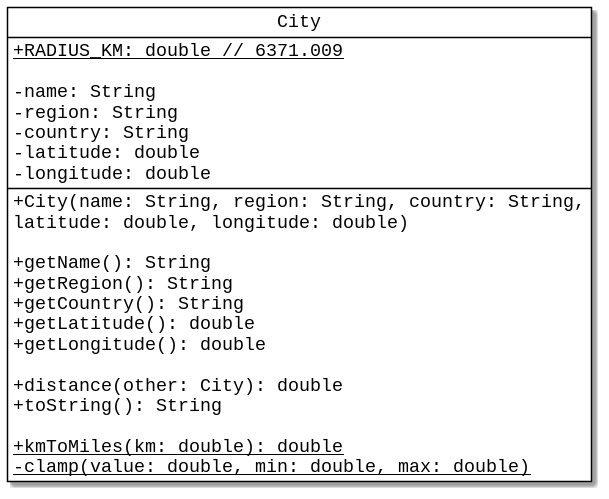
\includegraphics[scale=0.5]{figs/ch12/city.png}
\caption{UML Diagram for a City class}
\label{fig.cityuml}
\end{center}
\end{figure}

The class has private instance variables for the city name, its region (for the US, it's called a state; for Canada, it's a province; for Japan it's a prefecture), and its latitude and longitude measured in degrees.

This is an immutable class. (How would you determine this from the UML diagram?)

\java{RADIUS_KM} is a \java{static} \java{final} constant representing the radius of the earth in kilometers.

The constructor will make sure that the longitude is in the range -180 to 180 and the latitude in the range -90 to 90. The constructor will use the \java{clamp} method to enforce this:

\begin{code}
private static double clamp(double value, double min, double max) {
    double result = value;
    if (value <  min) {
        result = min;
    }
    else if (value > max) {
        result = max;
    }
    return result;
}
\end{code}


Questions: Why do you think this method was declared \java{private} instead of \java{public}? Why is it a \java{static} method instead of an instance method?

The \java{toString} method will display the information about the city; it can display the latitude and longitude as positive and negative numbers, or by using N, S, E, and W as abbreviations for north, south, east, and west. Display them to one decimal point. (Hint: \java{"\\u00b0"} is the degree symbol.) For example:

\begin{stdout}
San Jose, CA, USA: 37.3°, -121.9°
San Jose, CA, USA: 37.3°N, 121.9°W
\end{stdout}


The \java{distance} method will calculate the great circle distance between one \java{City} object and the \java{other} \java{City} object. Here is the formula where $r$ is the radius of earth in kilometers (6371.009), the first city's latitude and longitude are $lat_1$, $lon_1$ and the second city's latitude and longitude are  $lat_2$, $lon_2$:

\begin{equation*}
d = r\cdot cos^{-1}(sin(lat_1)\cdot sin(lat_2) + cos(lat_1)\cdot cos(lat_2)\cdot cos(lon_1 - lon_2))
\end{equation*}

{\bf Important}: The trigonometric functions all take their arguments as {\em radians}, not degrees. You can use the \java{Math.toRadians} method to convert degrees to radians:

\begin{code}
double degrees = 30.0;
double radians = Math.toRadians(degrees);
// Following line gives correct result (0.5)
System.out.println(Math.sin(radians));
\end{code}

The \java{main} method will set up an array of these \java{City} objects:

\begin{tabular}{|l|l|l|r|r|}
\hline
City & Region & Country & Latitude & Longitude \\ \hline
Antananarivo & Analamanga & MG & -18.93 & 47.52 \\ \hline
Brasilia & Distrito Federal & BR & -15.79 & -47.88 \\ \hline
Mumbai & Maharashtra & IN & 19.08 & 72.88 \\ \hline
Munich & Bavaria & DE & 48.08 & 11.57 \\ \hline
San Jose & California & US & 37.34 & -121.89 \\ \hline
Yokohama & Kanagawa & JP & 35.44 & 139.64 \\ \hline
\end{tabular}

The \java{main} method then prints a list of the cities and the inter-city distances with output as follows. Hint: use \java{"\%8.0f"} to round the distance to an integer:

\begin{stdout}
A: Antananarivo, Analamanga, MG (18.9°S, 47.5°E)
B: Brasilia, Distrito Federal, BR (15.8°S, 47.9°W)
C: Mumbai, Maharashtra, IN (19.1°N, 72.9°E)
D: Munich, Bavaria, DE (48.1°N, 11.6°E)
E: San Jose, California, US (37.3°N, 121.9°W)
F: Yokohama, Kanagawa, JP (35.4°N, 139.6°E)

Inter-city great circle distances in km:
        A       B       C       D       E       F    
A      ----
B      9991    ----
C      5052   13749    ----
D      8264    9214    6325    ----
E     17724    9716   13553    9459    ----
F     11399   17706    6720    9396    8356    ---- 
\end{stdout}

\end{exercise}

\begin{exercise}
Figure~\ref{fig.courseuml} is the UML diagram for a \java{Course} object that represents a college course. The \java{day} attribute gives the day on which the course is taught, with 1 representing Monday and 7 representing Sunday. The \java{startTime} and \java{endTime} are given as integers that represent military time (0000 is midnight and 2359 is 11:59 p.m.)

\begin{figure}[!h]
\begin{center}
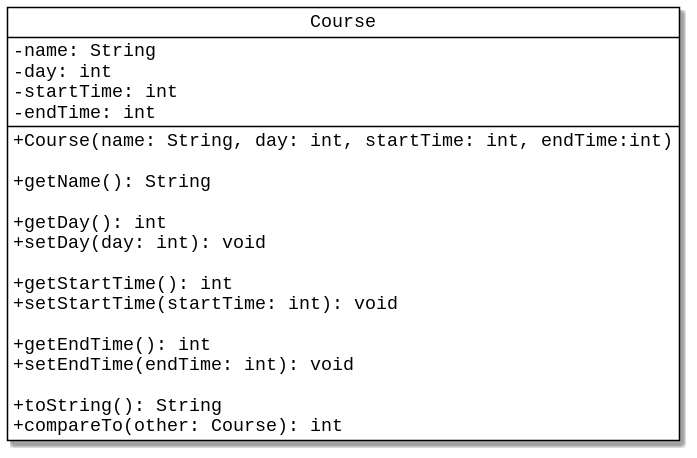
\includegraphics[scale=0.5]{figs/ch12/course.png}
\caption{UML Diagram for a Course object}
\label{fig.courseuml}
\end{center}
\end{figure}

When you write the constructor and the setters, make sure that the day of week is always in the range 1-7 and that the times are in the range 0000-2359. Make sure you handle a time like 2079 in some reasonable fashion---you decide what ``reasonable'' means here, and {\bf use comments to document it}. You may want to rewrite the \java{clamp} method from the preceding exericse to use integers as its parameters and return value. Then you can use it when writing a new \java{clampTime} method to enforce these conditions.

Note: a constructor can call an instance method; that is, the constructor for \java{Course} can call the \java{setDay}, \java{setStartTime}, and \java{setEndTime} methods. This will eliminate a lot of duplicated code.

The \java{compareTo} method uses the following criteria when doing a comparison: First, compare the \java{day} attributes. If they aren't equal, then return 1 or $-1$ (depending on which one is less or greater). If the \java{day} fields are equal, compare the \java{startTime} attributes and return 1, 0, or $-1$ depending on their relationship.

The \java{toString} method will display the course's attributes. Again, you decide what you want it to look like.

In the \java{main} method, create an array of the following courses, in this order. Note that ECON 010A has an invalid time so that you can test to see what your code does:

\begin{tabular}{|l|l|l|l|}
\hline
Name & Day & Start Time & End Time \\ \hline
ACCTG 001A & 1 & 1515 & 1645 \\ \hline
BIO 020 & 3 & 1235 & 1540 \\ \hline
COMSC 075 & 2 & 0915 & 1125 \\ \hline
ECON 010A & 4 & 1515 & 1679 \\ \hline
MATH 063 & 1 & 0915 & 1035 \\ \hline
PSYCH 018 & 3 & 1615 & 1750 \\ \hline
THEAT 034 & 1 & 1215 & 1335\\ \hline
\end{tabular}

Then, iterate through the array to find the courses with the earliest and latest start times according to the \java{compareTo} method.

\begin{minipage}[t]{0.8\textwidth}

\noindent\rule{\textwidth}{1pt}

{\bf NOTE:} You cannot do this in Java:
\begin{code}
int startTime = 0915;
\end{code}

The reason is that a leading zero indicates to Java that your number is {\em octal} (base 8), and there is no digit 9 in that number base. Instead, leave off the leading zero:

\begin{code}
int startTime = 915;
\end{code}

You do not have to worry about this when doing user input; the \java{nextInt} and \java{Integer.parseInt} methods use decimal (base 10) by default, so when a person enters the string \java{0915} it will be converted to integer without an error.

\noindent\rule{\textwidth}{1pt}

\end{minipage}

Sample output:

\begin{stdout}
Earliest course: MATH 063: M (0915-1035)
Latest course: ECON 010A: Th (1515-1659)
\end{stdout}

\end{exercise}
